\chapter{Background}
\index{Background@\emph{Background}}\label{background}%
In Section~\ref{back:phylogenetics}, I give a brief introduction to phylogenies and alignments and define basic definitions and concepts that will be used throughout my dissertation.  In Section~\ref{back:hmm}, I describe profile Hidden Markov Models (HMM) and their use in alignment estimation. Finally, in Section~\ref{back:app}, I describe applications of profile HMMs in the realm of phylogenetic placement, metagenomic analyses, and ultra-large alignment estimation.

\section{Phylogenetics}
\emph{Phylogenetics} is the study of the evolutionary relationships between different organisms.  A typical molecular phylogenetic study begins by collecting biomolecular sequences (DNA, RNA, or amino acid sequences) from the species of interest.  The evolutionary relationships between the different characters in the sequence are inferred through an alignment.  From the alignment, a tree representing the evolutionary history between the different species are estimated.  The steps of estimating an alignment and estimating a tree are core concepts used throughout my dissertation.  I now explain provide more details on the alignment and the tree, and on how one might go about estimating alignment and tree.

\paragraph{Tree: graphical model of evolution}\label{back:phylogenetics}
A \emph{phylogeny} is a graphical model that represents the evolutionary relationships between different species.  One of the most common representations is using a \emph{rooted tree} - a directed acyclic graph.  Each leaf in the tree represents a species, and each internal node in the tree represents a \emph{speciation event}.  Speciation events are the process in which one species give rise to new lineages of species.  The root of the tree represents the most recent common ancestor of all the species.  Throughout my dissertation, I will refer to the leaves of the tree as species, taxa, or sequences, interchangeably.  Similarly, I refer to phylogenies as trees, though a phylogeny does not necessarily have to be tree-like, and more complicated representations such as phylogenetic networks do exist~\cite{todo}.

Figure~\ref{back:phylo_tree}(a) shows an example of a rooted phylogenetic tree.  The relationship between the different species can be inferred from the tree.  For example, species $A$ and $B$ are more closely related than species $A$ and $C$ because $A$ and $B$ share a more recent common ancestor (red node) than $A$ and $C$ (blue node). The example shown is a rooted, i.e., the direction of evolution is known.  The root of the tree represents the most recent common ancestor (MRCA) of all the species (black node).  In general, estimating the root of the tree is very difficult as most common models used in phylogeny estimation assume time-reversibility, and under these models, it is not possible to determine which node is the ancestor and which node is the descendant.  Thus, when I discuss phylogenies, I refer to unrooted trees.

Figure~\ref{back:phylo_tree}(b) shows an unrooted version of Figure~\ref{back:phylo_tree}(a).  An unrooted tree is a \emph{binary} tree if all inner nodes have a degree of 3.  If an inner node has degree greater than 3, it is called a \emph{polytomy}.  Polytomies represent evolutionary relationships that cannot be resolved.  Figure~\ref{back:poly} shows an example of a tree containing a polytomy.  
%Polytomies arise when there is insufficient data to resolve the relationships between different organisms, or when rapid 
\textbf{Nam:Build polytomy figure}
\begin{figure}[htpb]
\begin{subfigure}[htpb]{\textwidth}
  \centering
  \includegraphics[width=0.60\linewidth]{{background/phylogeny}.pdf}\\
  \caption[]{A rooted phylogenetic tree.}
\end{subfigure}
\begin{subfigure}[htpb]{\textwidth}
  \centering
  \includegraphics[width=0.60\linewidth]{{background/unrooted_phylogeny}.pdf}\\
  \caption[]{An unrooted phylogenetic tree.}
\end{subfigure}
\caption[Example of rooted and unrooted trees.]{\label{back:phylo_tree} Example of a) a rooted phylogenetic tree, and b) the unrooted version of the same tree.  In the rooted tree, the red node is the MRCA of species $A$ and $B$, and the blue node is the MRCA of species $A$ and $C$.  The black node is the MRCA of all the species in the tree.  In the unrooted tree, the red edge represents the bipartition $\{CD|ABEFGH\}$.}
\end{figure}

\paragraph{Multiple Sequence Alignment.}
Biomolecular sequences are represented as character strings over an $n$-letter alphabet.  The most common alphabets are the 4-letter alphabets for nucleotides ($\{A,T,C,G\}$ for DNA and $\{A,U,C,G\}$ for RNA) and the 20-letter alphabet for amino acid sequences.  Because DNA is inherited from parent to child, biomolecular sequences are often used to reconstruct the evolutionary history of present day organisms.  

%However, the ancestral organisms that gave rise to the current species are lost, thus, the evolutionary history of present day sequences must be inferred from sequences collected in the present; 
%; sequences from ancestral populations are .  
\textbf{Should add some extra background on uses of MSA, functional annotation of proteins/environmental reads, detecting conserved domains in proteins, sequence database search, remote homology detection, phylogeny estimation, etc... so that way can motivate why MSA is important}

A fundamental step in understanding the relationship between the different sequences is to estimate an alignment on the sequences.  A \emph{Multiple Sequence Alignment} (MSA) is a data structure that represents the evolutionary relationships between the individual characters in a set of sequences.  An MSA on a set of sequences is defined by an $n x m$ matrix in which each row is a sequence that has been interspersed with gap characters (represented by ``-'').  Gap characters represent historical insertion and deletion events (called ``indel'' events).  Each column in the matrix represents a site of common evolutionary origin.  If a pair of characters descended from the same ancestral character, then they are called \emph{homologous} and will be in the same column in the MSA.  Homology is a transitive property, so if a nucleotide $A$ is homologous to nucleotide $B$ and $C$, then nucleotides $B$ and $C$ are also homologous to each other.  Figure~\ref{back:alignment} shows an example of a MSA.  The goal of an MSA is infer sites of shared homologies between the different sequences.

\begin{figure}[htpb]
\centering
\includegraphics[width=0.60\linewidth]{{background/unrooted_phylogeny}.pdf}\\
\caption[Example of a MSA.]{\label{back:alignment} Example of a MSA estimated on the sequence set $\{S1,..Sn\}$.  Originally the sequences are unaligned.  The sequences are aligned by inserting gaps into the sequences such that homologous characters line up in the same site.}
\end{figure}

\paragraph{Simulation study.}
There are many different methods for estimating an MSA and for estimating a phylogenetic tree.  As it is impossible to know the true history for a set of biological sequences, simulation studies are performed to test the performance of different alignment and phylogeny estimation techniques.

A typical molecular simulation study begins by generating a rooted model tree that represents the true evolutionary history of the set of sequences.  The model tree can be generated by using a phylogenetic tree from a previous study, or it can be generated by simulated a tree under a stochastic model of speciation events (see ~\cite{Aldous2001} for review of tree models).  Once a model tree has been generated, a stochastic model of sequence evolution is selected~\cite{todo}, as well as a model of indel events~\cite{todo}.  These models include parameters for the rate of substitutions as well as the rates of insertion and deletion events, and the a model for the length of the indel events.  Once all the parameters have been selected, a random sequence is generated at the root, and it is simulated down the model tree with substitution and indel events (see Fig.~\ref{back:seq_evo}).  The true sequence is known at each internal node, as well as the history of the mutation patterns.  Thus, at the very end of the simulation, the true MSA and true phylogeny of the sequences are known and can be used to compare the accuracy of MSA and phylogeny estimation methods. 

\begin{figure}[htpb]
\centering
\includegraphics[width=0.60\linewidth]{{background/seq_evolution_2}.pdf}\\
\caption[Example of sequence evolution.]{\label{back:seq_evo} Example of sequence evolution down a model tree.  The original sequence at the root is ``ATCG''.  Through a series of insertions (colored blue), deletions (colored red), and substitutions (colored green), the root sequence evolves to 4 new sequences. The goal of a molecular phylogenetic study is to infer from the unaligned sequences the true alignment and phylogeny.}
\end{figure}

\section{MSA estimation}\label{back:alignment}
Computing an MSA is typically formulated as an optimization problem of minimizing the differences between the sequences across the sites in the alignment.  One simple optimization metric used is the sum-of-pairs (SP) score~\cite{todo}.  The SP score is computed by summing the total number of mismatches (pairs of aligned ``non-gap'' characters that do not match) and indels (any ``non-gap'' characters aligned to a ``gap'' character) over all pairs of sequences in the MSA.  Figure~\ref{back:sp_score}a shows the computation of the SP score for a pair of sequences.  Figure~\ref{back:sp_score}b shows the SP score for two MSAs estimated on the same set of sequences.  In this example, the bottom MSA has a lower SP score and would be considered more accurate under the SP score optimization criterion.  

\begin{figure}[htpb]
\begin{subfigure}[htpb]{\textwidth}
  \centering
  \includegraphics[width=0.45\linewidth]{{background/sp_scoring}.pdf}\\
  \caption[]{Computing SP score for 2 sequences.}
\end{subfigure}
\begin{subfigure}[htpb]{\textwidth}
  \centering
  \includegraphics[width=0.60\linewidth]{{background/sp_score}.pdf}\\
  \caption[]{Computing SP score for an MSA.}
\end{subfigure}
\caption[Example of scoring MSAs.]{\label{back:sp_score} Example of a) computing the SP score for a pair of sequences, and b) the SP scores for two different MSAs of the same set of sequences.  In a), mismatches are highlighted red, and indels are highlighted blue.  The SP score is the sum of the total number of mismatches and indels.  In b) the SP scores for each pair of sequences are shown.  The total SP score for an MSA is the sum of all the pairwise SP scores.  In this example, the lower MSA has lower SP score and is more desirable under the SP score optimization criterion.}
\end{figure}

Computing an MSA that optimizes SP score (and many other similar metrics) is NP-complete~\cite{Wang1994,Bonizzoni2001} and thus, finding an exact solution is computationally intractable for large datasets.  Heuristics have been developed for MSA estimation(see~\cite{Notredame2002,Thompson2011} for survey and comparison of current methods), including progressive methods which build an MSA by progressively aligning pairs of sequences and then merging the alignments using an estimated tree~\cite{todo}, and iterative methods which combine progressive methods and iteration so that the estimated MSA from the progress step is reused to estimate a better MSA~\cite{todo}.  However, these methods suffer in that they do not scale linearly with the number of sequences to be aligned~\cite{Notredame2002}.

Another class of MSA estimation methods include methods that use profile Hidden Markov Models (HMM).  A profile HMM is a statistical representation of an MSA (see Section~\ref{back:hmm} for a more indepth overview).  HMM methods take an existing MSA and computes a profile HMM from that MSA.  Sequences are then independently aligned to the profile.  Thus, profile HMM methods scale linearly with the number of sequences to align to an existing MSA.  However, the quality of the HMM is heavily impacted by the quality of the existing MSA, and on datasets containing evolutionary divergent sequences, the ability for HMM methods to accurately detect homologies degrades~\cite{Moriyama2006,Finn2010}.

\paragraph{Quantifying error in alignments.}  If a true alignment is known via a simulation study, or a high quality curated alignment has been estimated, one can compare the error of an estimated alignment by examining the percentage of shared and missing homologies in the estimated alignment with respect to the reference alignment.

Three common metrics for quantifying the error of an estimated alignment are:
\begin{itemize}
\item \emph{sum-of-pairs false positive} (SPFP) rate - the total number of homologies in the estimated alignment that are not found in the true alignment, normalized by the total homologies in the estimated alignment,
\item \emph{sum-of-pairs false negative} (SPFN) rate - the total number of homologies in the true alignment that are not found in the estimated alignment, normalized by the total homologies in the true alignment, and
\item \emph{total column} (TC) error rate - the number of columns in the true alignment that are not exactly recovered in the estimated alignment, normalized by the total columns in the true alignment.
\end{itemize}

In my dissertation, I report SPFN and SPFP rates, as well as the arithmetic mean of the two rates.  In addition, I also report the TC error rate on protein datasets.  This metric is of interest when the goal is to examine how well alignment methods recover conserved domains in the protein alignment.

%One pair of metrics that can be used to score the error of an estimated MSA is the sum-of-pairs false negative (SPFN) and the sum-of-pairs false positive (SPFP) rates~\cite{todo}.  The SPFN rate is defined as the total number of homologies in the true alignment that are not found in the estimated alignment, normalized by the total homologies in the true alignment.  Similarly, the SPFP rate is defined as the total number of homologies in the estimated alignment that are not found in the true alignment, normalized by the total homologies in the estimated alignment.  


%As one might expect, estimating every single homology correctly at a site when there are many sequences is difficult for all but the most conserved sites.  

%\textbf{Build figure showing how SPFN and SPFP is computed}

\paragraph{Phylogeny estimation}\label{back:tree_estimation}
Many different methods (distance-based~\cite{todo}, parsimony-based~\cite{todo}, Bayesian methods~\cite{todo}, Maximum Likelihood methods~\cite{todo}(ML), as examples) exist for estimating a phylogenetic tree from an MSA (see~\cite{Huelsenbeck1995,Holder2003} for overview of current methods).  Of the current classes of methods, ML methods give better accuracy than distance-based and parsimony-based  methods~\cite{Kuhner1994}, and they are the only method can accurately scale to very large datasets~\cite{Liu2012,Price2010,Stamatakis2014}.  Thus I focus on ML-based methods for tree estimation for my dissertation.  

\textbf{Fill this out more.}

%Distance based methods such as Neighbor-Joining~\cite{todo} and UPGMA~\cite{todo} estimate a distance matrix based on the dissimilarity between the different sequences and attempt to find a tree such that the branch length distances between every pair of leaves closely reproduce the distances in the matrix.  Maximum parsimony methods~\cite{todo}

\paragraph{Quantifying error in trees.}  

Each edge in the tree defines a bipartition.  Trees on the same leaf set can be compared by examining the biparitions that they share in common and the bipartitions that are unique to each tree.  

For example, in Figure \ref{back:phylo_tree}(b), the red edge represents the bipartition $\{CD|ABEFGH\}$ (note that $\{CD|ABEFGH\}$ is identical to $\{ABEFGH|CD\}$).  Removal of this edge separates $CD$ from $ABEFGH$.  A tree can be uniquely identified by its set of bipartitions.  Thus, Figure \ref{back:phylo_tree}(b) can be uniquely identified by the bipartition set $\{\{AB|CDEFGH\}, \{CD|ABEFGH\}, \{EF|ABCDGH\},\{GH|ABCDEF\},$ $\{ABCD|EFGH\}\}$ (trival bipartitions that split a leaf node from the remaining leaves of the tree does not need to be listed as these bipartitions will be found in all trees that share the same leaf set).  Trees can be compared by examining the bipartition sets.

Three common metrics for quantifying the error of an estimated tree are:
\begin{itemize}
\item \emph{Robinson–Foulds} (RF) rate~\cite{RF} - the total number of bipartitions that are unique to the reference tree and estimated tree, normalized by the total bipartitions in both trees,
\item \emph{false positive} (FP) rate - the total number of bipartitions in the estimated tree that are not in found in the reference tree, normalized by the total bipartitions in the estimated tree, and
\item \emph{false negative} (FN) rate - the total number of bipartitions in the reference tree that are not in found in the estimated tree, normalized by the total bipartitions in the estimated tree.  The FN rate is also known as the missing branch rate.
\end{itemize}

For binary trees, $FN=FP=RF$.  My dissertation primarily reports the missing branch rate as the error metric for comparing trees.  For simulated datasets, the model trees are binary trees, thus reporting missing branch rate is identical to reporting the FP and RF rates.  For biological datasets, the reference trees are ML trees estimated on a curated alignment, with only highly support edges retained.  Thus, the reference trees on biological datasets are non-binary, and the FP and FN rates will differ.  It is extremely easy for a method to estimate a tree with low FP rate by random chance; the method could estimate a highly unresolved tree.  It is much more difficult for a method to estimate a tree with low FN rate by random chance.  Thus, reporting the FN rate for biological datasets is an appropriate measure. 

%For binary trees, $FN=FP=RF$.  For non-binary trees, these quantities The FN rate is also known as the missing branch rate as it is the percentage of branches that are missing from the estimated tree, and I will interchangeably use these two terminologies.  

%One metric that can be used to compare tree topologies is by looking at the total number of bipartitions that are unique to each tree.  This metric is known as the Robinson–Foulds (RF) distance~\cite{RF}.  More formally, let $S_1$ be the set of bipartitions in $T_1$ and $S_2$ be the set of bipartitions in $T_2$, then the RF distance is defined as: $RF=|S_1\cup S_2|-|S_1\cap S_2|$. Typically, this metric is normalized by the total number of bipartitions in $T_1$ and $T_2$.  

%If the true tree is known, then the error of an estimated tree can be measured by the percentage of bipartitions in the true tree that are not recovered in the estimated tree (the false negative rate), and by the percentage of bipartitions in the estimated tree that are not in found in the true tree (the false positive rate), and the average of these two rates (Robinson–Foulds rate).  More formally, if $T_1$ is the true tree and $T_2$ is the estimated tree, then the false negative (FN) rate is defined as: $FN=1-\frac{|S_1\cap S_2|}{|S_1|}$.  Similarly, the false positive (FP) rate is defined as: $FP=1-\frac{|S_1\cap S_2|}{|S_2|}$.  For binary trees, $FN=FP=RF$.  The FN rate is also known as the missing branch rate as it is the percentage of branches that are missing from the estimated tree, and I will interchangeably use these two terminologies.  



%\textbf{Nam: I need to provide more details on how reference trees are estimated on curated alignments, in particular cover carefully the bootstrap process so it's clear why reference trees are not resolved!}

Figure~\ref{back:tree_error} shows an example of a true tree and an estimated tree.  Each tree contains 5 bipartitions.  The bipartitions $\{AB|CDEFGH\}$ and $\{CD|ABEFGH\}$ are found in the true tree, but not present in the estimated tree.  Thus, the missing branch rate 20\%.  Similarly, the bipartitions $\{AC|BDEFGH\}$ and $\{BD|ACEFGH\}$ are found in the estimated tree, but are not present in the true tree, yielding an FP rate of 20\%.

%\textbf{Nam:  Add a little about non-binary trees, and that this dissertation focuses on FN rates because for simulation results FN=FP.  However, for biological datasets, we have bootstrap reference trees that are non-binary and so we focus on how well we can recover highly supported edges.  }

\begin{figure}[htbp]
\centering
{\includegraphics[width=0.60\textwidth]{background/unrooted_phylogeny_a}}
\caption[Computing error metrics of estimated tree.]{An example of the true tree and the estimated tree.  The estimated tree has an FN rate of $\frac{2}{5}$ (two bipartitions colored red in the true tree are not found in the estimated tree; five bipartitions in true tree) and has an FP rate of $\frac{2}{5}$ (two bipartitions colored blue in the estimated tree are not found in the true tree; five bipartitions in estimated tree).}  
\label{back:tree_error}
\end{figure}

\section{Profile Hidden Markov Models}\label{back:hmm}
A profile Hidden Markov Model (HMM) is a probabilistic model for representing an MSA.  
A profile HMM can be represented by a finite state machine (FSM, see Fig.~\ref{back:hmm_model}).  By transitioning through the FSM, a sequence can be generated from the HMM.  Similarily for a given sequence, the probability that the model generated the sequence can be computed which yields an alignment of the sequence to the HMM.   I now describe the FSM in more detail.

The FSM for a profile HMM consists of a start state $S$ and an end state $E$, a set of \emph{match states} $M=\{M_1,..,M_n\}$, a set of \emph{insertion states } $I=\{I_0,..,I_n\}$, a set of \emph{deletion states} $D=\{D_1,..,D_n\}$, and directed \emph{transition edges} $E=\{(M_i,M_{i+1}),(D_i,M_{i+1}),(I_i,M_{i+1}),(I_i,I_i)\}, i\epsilon \{1,..,n\}$.  Each transition edge has an associated probability, and the sum of all transition edges leaving a state must sum up to 1.  Each match and insertion state has an associated \emph{emmission probability vector} which is a probability that a character will exist at that state.

The match states represent contiguous columns (called ``consensus columns'') in the MSA.  In the simplest case, the match state $M_i$ models the column $c_i$ in the alignment.  Insertion states represent insertion events in the sequence.  Similarly, deletion states represent deletion events in a sequence.  If a sequence contains no indels (i.e., it aligns perfectly to the MSA without the need of inserting any gaps), then the path through the model would proceed from match state to match state.  However, if the sequence contains an insertion event at the second character, then the path through the FSM would go from match state $M_2$ to insertion state $I_2$, and would remain at insertion state $I_2$ until all the estimated insertion characters have been processed, at which it goes to the next match state.  Finally, if the sequence seems to be missing a character relative to the MSA, then a deletion event has occurred.  For example, if the first and second characters in the sequence are $AA$, but the first 3 columns in the MSA contain with $ATA$, then this suggest that the sequence had a deletion event of the second column.  In this case, the path through the FSM would go from $M_1$ to $D_2$ to $M_3$.  

\textbf{Need to clean up the text on the HMM, it's too confusing right now, maybe more explain diagrams/figures, or maybe I am giving too much details, but still not enough}

The process of aligning a sequence to a profile HMM is to find the most probable path through the FSM for generating the sequence.  This can be solved via the Viterbi dynamic programming algorithm~\cite{Viterbi1967} in $O(L*|M|^2)$ time complexity, where $L$ is the length of the sequence and $|M|$ is the total number of match states.  Thus, alignment using a profile HMM grows linearly with the number of sequences to align.

\textbf{Add more details to sequence alignment, maybe show graphical example}

%For example, if the first column in the MSA contains $\{ATTT-\}$, then there would be a match state $M_1$ with an associated emmission probabilities vector $\{P(A)=0.25;P(T)=0.75;P(C)=P(G)=0\}$.   
%Each match and insertion state has an associated \emph{emmission probability vector} which is a probability distribution of the character that will be emmitted upon leaving the state.  So if a column contains many $A$s, then the emmission probability for $A$ in the associated match state will also be high.

%The match states model the distribution of the characters for a set of contiguous columns in the MSA.  In the simplest case, the match state $M_i$ models the column $c_i$ in the alignment, though a contiguous set of very gappy columns may be collapsed into a single match state.  For example, if the first column in the MSA contains $\{ATTT-\}$, then there would be a match state $M_1$ with an associated emmission probabilities vector $\{P(A)=0.25;P(T)=0.75;P(C)=P(G)=0\}$.   

%Insertion states allow insertions to occur before and after each match state.  .  Deletion states represent deletions in the  

%Each match state $M_i$ has a transition probability to $M_{i+1}$ which represents 
%In the most simple representation of an MSA, each column $c_i\element{c_1,..c_n\}$ in the MSA maps to the match states.  

\begin{figure}[htbp]
\centering
{\includegraphics[width=0.75\textwidth]{background/hmm}}
\caption[Profile HMM representation of an MSA.]{Profile HMM representation of an MSA using a finite state machine.}  
\label{back:hmm_model}
\end{figure}

% \begin{figure}[htbp]
% \centering
% {\includegraphics[width=0.80\textwidth]{sepp/hmmer_papara}}
% \caption[Comparison of HMMALIGN+pplacer and PaPaRa+pplacer.]{Comparison of HMMALIGN+pplacer and PaPaRa+pplacer under 3 different model conditions, ranked in order of increasing rate of evolution.  Thus, M4 is the slowest evolving dataset, and M2 is the fastest evolving dataset.  The number of sequences in the backbone set is 500 for all model conditions.} 
% \label{background:initial}
% \end{figure}
\section{Applications of profile HMMs}\label{back:app}
\subsection{Phylogenetic placement}
As I briefly mentioned in Chapter~\ref{intro}, phylogenetic placement is a method for inserting query sequences into an existing phylogenetic tree.  Phylogenetic placement is an alternative approach to phylogeny estimation for inferring the phylogenetic relationship between a set of query sequences and a set of full-length sequences in the existing tree.  Rather than estimating a new phylogenetic tree on the entire set of full-length and query sequences, phylogenetic placement infers the relationships between the query sequence and the full-length sequences one at a time, making the computational complexity of placement grow linearly with the number of query sequences.  In addition, if new query sequences are added, the placement algorithm needs to be run on just the new sequences.  Phylogeny estimation, on the other hand, would have to be re-run on the entire set of sequences every time a new sequence is added.  

Phylogenetic placement is extremely advantageous in the analyses of short DNA fragments taken from an environmental sample
%~\cite{todo} 
where there can be potentially millions of fragmentary reads.  By placing a short read from an unknown species into a taxonomic tree, one can infer the taxonomic classification of the read based on its placement within the taxonomic tree.  

%

I now formally describe the phylogenetic placement problem as follows:

%\textbf{Add text before the formal description on why phylogenetic placement is necessary.  Good for analyzing short fragmentary reads because most traditional alignment methods assume global alignment, need local alignment for shorter fragments.  In addition, under the context of AToL, can build a large tree by aligning to only a backbone alignment instead of all sequences against all other sequences, and then inserting into an existing tree instead of estimating an entire tree on all sequences.  Thus phylogenetic placement may be a method for getting at a tree of all life.}
%This method is useful in the analyses of short fragmentary reads.  When a dataset consists of sequences of heterogeneous lengths containing both full-length and fragmentary sequences, attempting to globally align the sequences together may result in very gappy alignments of the fragmentary reads.  A better approach is to estimate an alignment and tree on the full-length sequences, and then insert the remaining fragmentary sequences into tree.  The advantage

%Many traditional alignment techniques perform global alignment and assume all the sequences are full-length and of roughly equal size.  When this assumption is violated, such as in the case of aligning fragmentary reads, global alignment methods may end up inserting many gaps to get the fragmentary sequence to align well to the full-length sequences~\cite{todo}.  

\noindent{\em Phylogenetic Placement Problem. }
\begin{itemize}
\item Input: the alignment $A$ and tree $T$ estimated on a set $S$ of full-length sequences (called the {\em backbone} tree and {\em backbone} alignment) and query sequence $s$.
\item Output: tree $T'$ containing $s$ obtained by adding $s$ as a leaf to
$T$.
\end{itemize}

Several methods have been developed for this problem using
the following two steps:

\begin{itemize}
\item Step 1: align $s$ to the backbone alignment $A$ to produce the alignment $A'$, called the {\em extended alignment}
\item Step 2: insert $s$ into $T$ using $A'$, optimizing some criterion
\end{itemize}
Methods for the first step 
include HMMALIGN~\cite{Eddy1998}, PaPaRa~\cite{Berger2011a}, Mafft-profile~\cite{Katoh2012}, and PAGAN~\cite{Loytynoja2012}.  
Methods for the second step include EPA (run within RAxML)~\cite{Berger2011} and pplacer~\cite{Matsen2010}, both of which
seek to optimize maximum likelihood
(pplacer also provides a Bayesian approach), and MLTreeMap~\cite{Stark2010}, which can optimize either ML or Maximum Parsimony (MP).  In~\cite{Stark2010}, Stark and Berger found that optimizing ML resulted in overall better placements, albeit with an increase in running time.

Phylogenetic placement methods can be described by the methods used for the alignment and placement steps.  Three such methods include PaPaRa+EPA~\cite{Berger2011}, HMMALIGN+EPA~\cite{Berger2011a}, and HMMALIGN+pplacer~\cite{Matsen2010}.  As EPA and pplacer both optimize likelihood, they were found to have almost identical 
placement accuracy, but have somewhat
different memory usage and algorithmic features~\cite{Matsen2010}.

%hence the differences between HMMALIGN+EPA and HMMALIGN+pplacer
%do not impact the placement accuracy.

The two techniques for computing the extended alignment,
PaPaRa and HMMALIGN, are very different.  HMMALIGN requires only a backbone alignment to align the query sequences.  PaPaRa, on the other hand, is a phylogeny aware method and requires both a backbone alignment and backbone tree to align the query seuqneces.
HMMALIGN computes a profile HMM to represent the MSA, and then aligns the query sequences to the HMM.  In contrast,
PaPaRa uses RAxML to estimate ancestral state 
vectors at all candidate insertion points on every edge of the 
tree, aligns the query sequence to every ancestral state
vector, selects the alignment that had the best score, and uses
it to extend
alignment $A$ to include $s$.  Thus, PaPaRa is more computationally expensive as it depends on both the number of query sequences to align and on the size of the backbone tree.  In~\cite{Berger2011a}, Berger and Stamatakis found that 
PaPaRa+EPA had better placement accuracy on large backbone trees or on short query sequences.  For small backbone trees or on longer query sequences, HMMALIGN+EPA had better placement accuracy.  

However, the improvement in topological accuracy reported~\cite{Berger2011a} for
PaPaRa+EPA over HMMALIGN+EPA was
relatively small, with PaPaRa+EPA placing
query sequences on average
about one edge closer to the correct
location, out of 799 edges. 
Therefore, PaPaRa+EPA and HMMALIGN+EPA are very close
in terms of placement accuracy, although substantially different
in terms of running time (PaPaRa anywhere from 6 to 43 times slower).  

\paragraph{Comparing placement accuracy.}  
The metric used in my dissertation for measuring the accuracy of placement is the change in missing branch rate of the backbone tree before and after insertion of the query sequence (called \deltafn ).  More formally, if $FN$ is the number of missing branches in the backbone tree $T$, and $FN'$ is the number of missing branches in $T'$, then \deltafn$=FN'-FN$.  Note that unlike $FN$ rate used in reporting tree error for phylogeny estimation, \deltafn is not normalized and thus is actual change in the number of missing branches.  Figure~\ref{back:placement_error} shows an example of this computation.  Let the initial backbone tree have 0 FN.  After the insertion of the query sequence $s$ into $T$, $T'$ is missing bipartitions $\{As|BCDEFGH\}$ and $\{ABs|CDEFGH\}$ (bipartitions colored red in Fig.~\ref{back:placement_error}).  The resulting \deltafn~is 2.

%\textbf{Nam: discuss possible case of \deltafn~ being negative.}

\begin{figure}[htbp]
\centering
{\includegraphics[width=0.60\textwidth]{background/unrooted_phylogeny_b}}
\caption[Computing \deltafn~error of query sequence placement.]{\label{back:placement_error}An example computing the \deltafn~error of query sequence placement.  The backbone tree originally has 0 missing branches.  After insertion of the query sequence $s$, the estimated tree $T'$ is missing 2 bipartitions that are found in the true true (missing edges colored red).  Thus, the \deltafn~is 2.}
\end{figure}

\subsection{Metagenomic analyses}\label{back:metagenomic}
Traditionally, bacterial species of interest from an environmental sample were identified by first culturing a clonal colony of the unknown species in a laboratory environment, and then sequencing the genetic material directly from the colony.  As the genetic material came from a single species and the Sanger sequencing technology used resulted in read lengths of 800bps with roughly 20,000 to 200,000 reads~\cite{todo}, assemblying the reads into longer contigs was computationally feasible on a desktop machine.  From the contigs, the bacteria genome could be assembled and the species could be identified.

However, an estimated 99\% of all microbial life cannot be cultured in lab~\cite{todo}, and thus, the majority of bacterial life cannot be studied using this pipeline.  One method to analyze microbial life without the need to grow them in the lab is through \emph{metagenomic}.  Metagenomics is the study of genetic material taken directly from an environmental sample.  By examining the DNA sequences from a metagenomic sample, we can identify the species present in the sample, as well as estimate the relative abundances of the species.

Metagenomic analyses are not without its difficulties.  Unlike the traditional approach to taxonomic identification where reads are generated from a clonal colony, the reads generated from a metagenomic sample do not all come from a single species.  In addition, the sequencing technology used typically generates much shorter reads than Sanger reads (80 to 100bps for Illumina reads), and there can be millions of sequences.  Thus, a fundamental challenge in a metagenomic analyses is classifying the potentially millions of short reads with taxonomic labels.

Classifying the metagenomic sequences requires
extrapolating the knowledge contained in sequence databases to
previously unseen DNA strings.  Simple similarity-based approaches
(e.g., picking the best database hit as the best `guess' at the
taxonomic label) have been shown to be insufficiently
accurate \cite{closest-blast-hit}, leading to the development of 
new and more sophisticated methods.

Recently developed methods improving
on the simple similarity-based approaches include 
(a) composition-based approaches that rely on
various machine learning techniques 
(Support Vector Machines in
PhyloPythia and PhyloPythiaS \cite{McHardy2007a, Patil2011}, 
Interpolated Markov Models in Phymm 
\cite{Brady2011},
Bayesian models in NBC \cite{Rosen2011}, or neural networks~\cite{SOM2006}) to
classify sequences based on their DNA composition (usually based on
the frequency of short k-mers),
(b)  more sophisticated analyses of
similarity search results (e.g., using least-common-ancestor
aggregation in Megan \cite{Huson2007}, or classifiers built from similarity
search results as done in MetaPhyler \cite{Liu2011d,Liu2011}, 
MetaPhlAn \cite{Segata2012a}, and mOTU \cite{Sunagawa2013}
or protein profiles in Carma \cite{Gerlach2011b}), and
(c) combinations of
multiple approaches (e.g., composition and similarity based approaches
in PhymmBL \cite{Brady2009}).  
Some of these approaches (e.g., most of the
composition-based approaches) can be applied to any DNA sequence,
while others are specific to a reference collection of carefully
selected genes (e.g., MetaPhyler, MetaPhlAn, and mOTU use a collection of
universal or clade-specific marker genes).  These
``marker-gene" methods can
achieve much higher recall than other
approaches~\cite{Liu2011d} for sequences from the marker genes, but 
can only classify a small
fraction of all sequences (namely, those that match the 
selected marker genes). 

Abundance profiling, also called ``phylogenetic profiling", 
seeks to estimate the relative
abundance of the species (or
genera, or families, etc.) within a sequence dataset.
While many methods produce these estimates by characterizing
most (or all) of the sequences in the dataset, marker-based methods
produce these estimates by characterizing only those
sequences that match the marker genes they rely on.
Since the marker genes are supposed to be single
copy and universal, these estimations do not need to
be corrected for the copy number in each genome, or for
missing data. 
However, the restriction to sequences that match the marker genes
has the potential to reduce accuracy since it means only a subset
of the sequences are characterized.

\paragraph{Taxonomic identification}\label{back:taxonomic_id}

\paragraph{Taxonomic profiling}\label{back:taxonomic_profiling}



% Metagenomic studies of microbial communities commonly generate
% millions to hundreds of millions of sequencing reads.  The assignment
% of accurate taxonomic labels to these sequences is a critical
% component in many analyses, but is
% complicated by the fact that the majority of the organisms
% found in environmental or host-associated communities cannot be easily
% cultured in a laboratory, and an even smaller number have been
% sequenced, even partially.  Thus, these commonly encountered organisms
% are largely absent from existing databases of known genomes and genes.
% Providing taxonomic labels to metagenomic sequences requires
% extrapolating the knowledge contained in sequence databases to
% previously unseen DNA strings.  Simple similarity-based approaches
% (e.g., picking the best database hit as the best `guess' at the
% taxonomic label) have been shown to be insufficiently
% accurate \cite{closest-blast-hit}, leading to the development of 
% new and more sophisticated methods.
% 
% Recently developed methods improving
% on the simple similarity-based approaches include 
% (a) composition-based approaches that rely on
% various machine learning techniques 
% (Support Vector Machines in
% PhyloPythia and PhyloPythiaS \cite{McHardy2007a, Patil2011}, 
% Interpolated Markov Models in Phymm 
% \cite{Brady2011},
% Bayesian models in NBC \cite{Rosen2011}, or neural networks~\cite{SOM2006}) to
% classify sequences based on their DNA composition (usually based on
% the frequency of short k-mers),
% (b)  more sophisticated analyses of
% similarity search results (e.g., using least-common-ancestor
% aggregation in Megan \cite{Huson2007}, or classifiers built from similarity
% search results as done in MetaPhyler \cite{Liu2011d,Liu2011}, 
% MetaPhlAn \cite{Segata2012a}, and mOTU \cite{Sunagawa2013}
% or protein profiles in Carma \cite{Gerlach2011b}), and
% (c) combinations of
% multiple approaches (e.g., composition and similarity based approaches
% in PhymmBL \cite{Brady2009}).  
% Some of these approaches (e.g., most of the
% composition-based approaches) can be applied to any DNA sequence,
% while others are specific to a reference collection of carefully
% selected genes (e.g., MetaPhyler, MetaPhlAn, and mOTU use a collection of
% universal or clade-specific marker genes).  These
% ``marker-gene" methods can
% achieve much higher recall than other
% approaches~\cite{Liu2011d} for sequences from the marker genes, but 
% can only classify a small
% fraction of all sequences (namely, those that match the 
% selected marker genes). 
% 
% Abundance profiling, also called ``phylogenetic profiling", 
% seeks to estimate the relative
% abundance of the species (or
% genera, or families, etc.) within a sequence dataset.
% While many methods produce these estimates by characterizing
% most (or all) of the sequences in the dataset, marker-based methods
% produce these estimates by characterizing only those
% sequences that match the marker genes they rely on.
% Since the marker genes are supposed to be single
% copy and universal, these estimations do not need to
% be corrected for the copy number in each genome, or for
% missing data. 
% However, the restriction to sequences that match the marker genes
% has the potential to reduce accuracy since it means only a subset
% of the sequences are characterized.

% \paragraph{Taxonomic identification through phylogenetic placement.}
% One approach toward taxonomic identification is through phylogenetic placement.  The evolutionary relationship between the the query sequence and the backbone sequences can be inferred from the placement location.  For example, in Figure~\ref{tipp:placement}, $Q1$ is placed closest to Species $A1$, and thus, it can be inferred that $Q1$ is more closely related to Species $A1$.  Similarly, $Q2$ is more closely related to Species $A1$ and $A2$ than to Species $B1$ and $B2$.  Thus, one simple technique for identifying a query sequence is to classify it by the LCA of its sibling leaf nodes.  Thus, $Q1$ would be classified as Species $A1$ (its only sibling leaf node is Species $A1$) and $Q2$ would be classified as Genus $A$ (its sibling leaf nodes are Species $A1$ and Species $A2$).  
% 
% \begin{figure}[htpb]
% \begin{center}
% {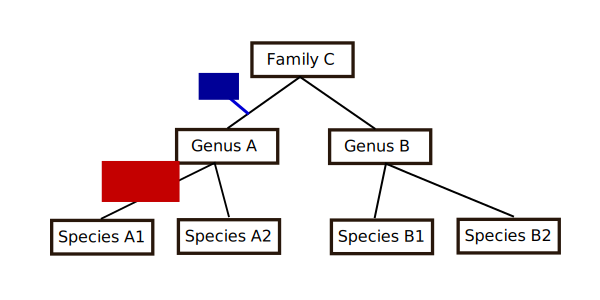
\includegraphics[scale=0.8]{tipp/placement.pdf}}
% \end{center}
% \caption[Taxonomic classification using phylogenetic placement]{\label{tipp:placement} Taxonomic classification using phylogenetic placement.  The leaf nodes of the rooted backbone tree are labeled with the species name.  Each query sequences is placed onto an edge in the backbone tree and is classified by the LCA its sibling leaf nodes.}
% \end{figure}
% 
% Using this approach, I compared SEPP and HMMALIGN+pplacer for taxonomic identification under a \emph{leave-species-out} experiment.  Under a leave-species-out experiment, the species of the query sequence is removed from the backbone alignment and tree, simulating the classification of a novel species.  Thus, while the species of the query sequence cannot be correctly identified, the remaining taxonomic lineage (genus, family, etc...) can still be correctly classified.  The fragments were simulated under differring models and rates of sequencing error.  
% 
% Figure~\ref{tipp:preliminary_sepp} shows that SEPP is more sensitive than HMMALIGN+pplacer under the hardest model condition (``454\_3''), classifying more fragments correctly, especially at the phylum level.  Both methods tend to classify the large majority of the fragments, leaving very few fragments unclassified.  This results in a very high false positive rate, especially under more difficult conditions.  
% 
% To understand why this is the case, it's important to note that pplacer outputs multiple possible locations for the placement of each query sequence.  Each placement has an associated with a likelihood weight ratio.  However, when HMMALIGN+pplacer or SEPP is used for taxonomic classification, only the placement with the likelihood weight ratio is used, ignoring that there may be other placements with almost as high weight.  This was one of the key insights in the development of TIPP.  By taking into account different sources of uncertainty, both in alignment and placement, the false positive rate could be reduced.

% \begin{figure}[htpb]
% \begin{center}
% {\includegraphics[scale=0.4]{{tipp/sepp.species}.pdf}}
% \end{center}
% \caption[Comparing SEPP and HMMALIGN+pplacer for taxonomic identification]{\label{tipp:preliminary_sepp} Leave-species-out experiments comparing SEPP and HMMALIGN+pplacer taxonomic classification accuracy on the rpsB gene under sequences simulated under different error model conditions.  Fragments were simulated with either Illumina-like or 454-like errors, and with varying rates of error.  Models denoted with a ``1'' have the lowest rates of error, and models with a ``3'' or ``4'' have the highest rates of error.  SEPP is run using a alignment decomposition size of 100 and placing on the entire backbone tree.}
% \end{figure}

%Taxon identification methods only classify a
%subset of the fragments (some correctly and some incorrectly), and
%will leave some fragments unclassified at each taxonomic level.
%Therefore, evaluations of taxonomic classification methods
%consider the percent of fragments classified
%at each rank correctly, incorrectly, or unclassified.  

%However, accurate classifications of just the fragments matching
%marker genes is sufficient for many purposes.
%For example, most culture-independent
%studies of microbial communities have relied on the
%analysis of the 16S rRNA gene.
%These studies, generating broad taxonomic profiles of the
%communities being studied, have been the basis for
%many important discoveries in microbial ecology and
%biomedicine  \cite{Turnbaugh2009}. % Alternative: Aagaard2012, Belda-Ferre2012
%In addition, 
%taxon identification methods should accurately label
%sequences already found in public databases, but should also provide accurate
%guesses on the taxonomy of sequences that are only distantly related
%to known sequences.  In fact, identifying novel organisms or taxonomic
%clades is an important focus of recent studies~\cite{eisen} and taxon
%identification software should be able to accurately identify putative
%novel organisms.  


% We have developed TIPP, a new method for taxon
% identification and phylogenetic profiling.
% TIPP is a marker-based method, but can be used to
% characterize any sequence matching any gene for which
% a dense enough sample of full-length sequences are
% available. In this paper, we explore TIPP using the
% Metaphyler's collection of 30 marker genes.

%\subsection{Ultra-large alignment estimation}\label{back:ultra_large}
